\section{How is Abstraction Used in Creative Work?}

One definition of abstraction is that higher-level features are stable and static whereas lower-level features are those that can change in context \cite{shapira2012levels}. From an information storage perspective, high-level abstractions form units of information, or chunks, formed from recognized patterns \cite{Chase1973,Gobet2001,Gobet1998}. Early in creative work, higher-level abstractions enable the exploration of concepts rather than details such as when dancers use marking to think through an overall choreography \cite{kirsh2011marking} or when illustrators or designers use preliminary sketches to communicate rough thoughts \cite{Buxton2007, landay1996sketching, Tversky2011,Tversky2009}. Rubrics and templates are other forms of abstraction tools because they highlight structural goals that are adapted and refined through the addition of concrete details \cite{andrade2005teaching,yuan2016}. While experts utilize abstraction techniques like sketching to explore and engage in a reflective dialogue with others and their work \cite{schon1984reflective,Tversky1999,Tversky2009}, novices are often drawn to details \cite{jansson1991design,marsh1996examples,Smith1993}. Particularly in visual creative work, this may be because novices are hesitant of their drawing ability or perceive even sketching to be more permanent \cite{Hennessey,welch2000sketching}. This chapter presents abstraction blocks as a strategy for malleable, high-level chunking in visual creative work that eliminates the necessity for early-stage sketching. 

\subsection{Limited Support for Abstraction in Collaborative Creative Tools}
%TOOLS FOCUS ON DETAILS INSTEAD OF ABSTRACTION
Particularly for online collaboration in creative work, tools and strategies for abstraction are limited. Many online projects take a crowdsourcing workflow approach, breaking down larger projects into smaller microtasks with a global goal to ensure coherence even in asychronous collaborations \cite{Hahn2016}. For text-based projects such as writing a collaborative story, workflows that decompose the work into concrete chunks and allow for interdependent contributions can facilitate structured, high-quality work \cite{Kim2016,Kim2017,Retelny2014,Salehi2018,Valentine2017}. Visual creative work like drawing is similar to that of written work in that an overall theme and composition need to be developed to create a cohesive final artifact, but while text has inherent sequential structure, images are not linear and not as easily broken down into independent workable parts \cite{Johnson-Laird1983}. 

Communication of abstract ideas within these collaborations may rely more on coordinating actions and developing rapport \cite{Davis2017,Davis2016}, which can be difficult in online settings where groups must rely on technological affordances to effectively communicate \cite{Hollan1992,Jensen2018}. Strategies for abstraction in collaborative visual work are limited in implementation. For example, SwarmSketch \cite{swarm} allows users to influence the direction of a collaborative drawing by contributing a single ink stroke however they like, but does not provide tools for communication between contributors or structure for how work should be coordinated. As a result, many drawings become a haphazard collection of strokes that no longer match the original goal and are difficult to change \cite{Boxer2005}. The Johnny Cash Project \cite{TheJohnnyCashProject2012} also predefines the overall project goal of collaboratively making a hand-drawn music video and coordinates contributor work through individual tasks (such as tracing over a designated image); however, it necessarily limits contributions to a single level of detail for ease of coordination, preventing contributors from influencing the direction of the project as a whole. 

\begin{figure}
\centering
  %\vspace{-0.2in}
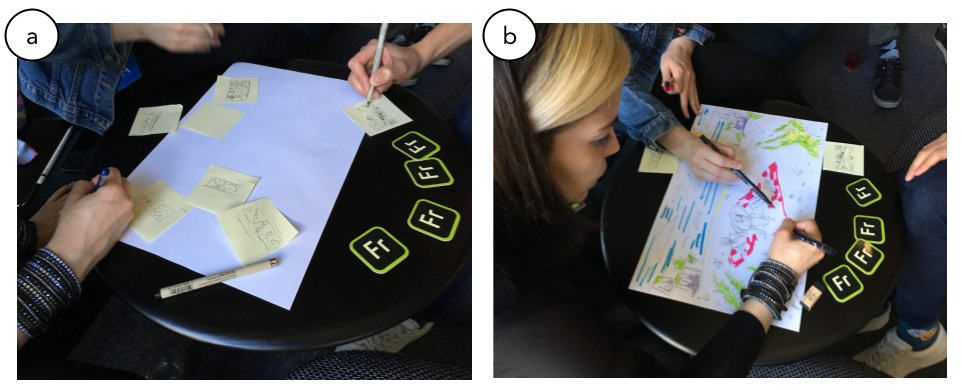
\includegraphics[width=\textwidth]{abstraction/figures/expert.png}
\vspace{-0.2in}
  \caption{a) Experts started planning by sketching multiple thumbnails that conveyed overall structure and composition more than details. b) These composition sketches provided a reference for experts during drawing.}
  ~\label{fig:expert}
  \vspace{-0.2in}
\end{figure}

``Blank page'' tools allow for open-ended abstraction, but are often unstructured. The problem with remaining too abstract or unstructured, especially in collaborative work, is that communication and consensus may get lost in the woods \cite{hinds1999curse,hinds2001}. Multiplayer experiences such as those in  Figma (www.figma.com), Google Docs \cite{wang2015students}, or collaborative drawing canvases (www.drawpile.net) enable a large range collaboration strategies, from allowing anyone to modify anything through pixel-perfect editing, to splitting the canvas or document into sections and assigning collaborators to each part. Digital whiteboards \cite{Ishii1992} and sketch interfaces \cite{lin2000denim} similarly give users the freedom to express their thoughts with as much or as little detail as desired. However, these systems leave it to the users to develop their own external collaboration structures. Without prerequisite knowledge of abstraction strategies, novices especially may continue to lean towards specific details, such as the exact specifications of a sketch \cite{welch2000sketching} or precise wording of an essay \cite{sommers1980revision}. Abstraction blocks ground the exploration and communication of abstract ideas to movable boxes to shift focus away from low-level details while giving tangible artifacts with which to interface.
